\section{Grundlagen, Stand der Forschung} 
\subsection{Adversarial Attacks}

Adversarial Attacks sind ein faszinierendes Phänomen im Bereich des Deep Learning, das in den letzten Jahren zunehmend an Bedeutung gewonnen hat. Diese Angriffe beziehen sich auf gezielte Manipulationen von Eingabedaten, die darauf abzielen, neuronale Netzwerke zu täuschen und falsche Vorhersagen zu erzwingen. Sie werfen wichtige Fragen zur Robustheit und Sicherheit von Deep Learning Modellen auf und haben weitreichende Implikationen für deren praktische Anwendungen \cite{goodfellow_explaining_2015}. 

\subsubsection{Grundlagen} 

Die Abbildung \ref{fig:grundlagen} illustriert den allgemeinen adversarial Attacke auf ein beliebiges Model $c$. 

\begin{figure}[H]
    \centering
    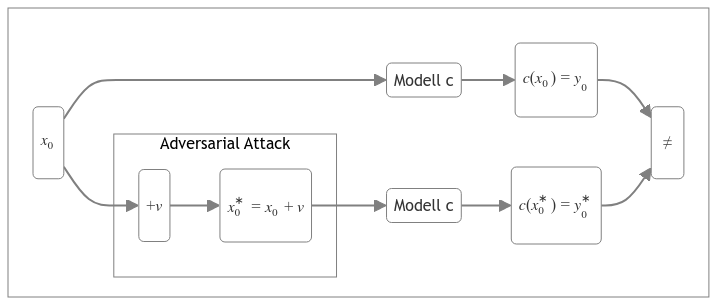
\includegraphics[width=13.5cm]{01-images/02-grundlagen/adversarial-attack.png}
    \caption{Vorgang einer Attacke}
    \label{fig:grundlagen}
\end{figure}

\begin{itemize}
    \item $x_0$, ist der Eingabewert, dies kann ein Signal, Bild oder sonstige Formate sein.
    \item $v$, ist die Perturbation, die Störung.
    \item $x_0^{*}$, der veränderte, attackierte Eingabewert durch die Perturbation.
    \item $c$, Das Modell, welche die Eingabe verarbeitet und Output generiert.
    \item $y_0$, Output des Modells durch den unveränderten Eingabewert.
    \item $y_0^{*}$, Output des Modells durch den attackierte Eingabewert.
    \item $\neq$, der Output von $y_0$ und $y_0^{*}$ ist nicht gleich.
\end{itemize}


\subsubsection{Allgemeine Beispiele für Adversarial Attacks} 

\todo{adversarial tshirt}

\subsubsection{Adversarial Attacks auf Bildklassifikation} 

Bei Adversarial Attacks auf Bildklassifikationsmodelle werden die Eingabewerte durch eine minimale Veränderung modifiziert, die vom menschlichen Auge nicht mehr wahrnehmbar ist.

\subsection{Universal Adversarial Attacks auf Bildklassifikation} 

Bei der Universal Adversarial Attacks wird eine "Universelle" Perturbation erzeugt, welches mehrere Modelle und unabhängig vom Datensatz auf alle Bilder addiert werden kann und das Modell somit zu einer Fehlklassifikation geschieht. 

\subsubsection{Grundlagen}

\subsubsection{Unser Hauptpaper}

Unser Hauptpaper "Universal adversarial perturbations" \cite{moosavi-dezfooli_universal_2017} dient als unsere Vorlage dieser Bachelorarbeit, auf die wir unsere Arbeiten stützen. 

\subsubsection{Bisherige Herausforderungen bei der Verteidigung}

